\chapter{INTRODUCTION}
\label{chap:intro}

%intro here in one paragraph

The approach of enormous informational collections has put weight on the Mathematics and Statistics people group to reexamine how to apply conventional of investigation and inferencing. Both atmosphere and oceanographic science disciplines are feeling this information blast and are attempting to scale. Extraordinary measures of information are made accessible by administrative offices like \gls{nasa} and \gls{noaa}, and vigorously utilized by mainstream researchers to draw inductions. The customary perception and conveyance instruments can be enhanced to deal with a flood of new information conveyance. The methods used to envision and recover these information should be rethought. Worldwide expectations require current mobile application innovations for expert and novice to imagine and get information rapidly, precisely, and as effortlessly on their hands as could be expected under the circumstances.

Conventional strategies for parsing through a remote/nearby document of records, choosing significant documents, opening the documents and performing examination on a solitary \gls{pc} don't scale with enormous information. Researchers are investing more energy exploring through information as opposed to discovering disclosures. More awful still, beginners as youngsters, specialists, understudies and potential researchers get baffled and abandon utilizing these rich informational indexes. Toolboxes web applications and of course mobile applications are recommended in this proposal to alleviate this weight. Present day \gls{restfull} application configuration gives the network a mobile stick to enable them to swim through the huge information soil.


\section{Background and significance of visualizing spatial data using smart phones}

The fields of Geo-information innovation and cartography have seen sensational changes in the last decade. In prior days \gls{gis} have been an instrument of specialists as opposed to the majority and requested top of the line machines and numerous abilities to run them. In the mid nineties the work area \gls{gis} appeared, which was anything but difficult to utilize and encourage with the Internet and Web mapping, Geo-information ended up famous among ordinary citizens. After the great achievement of the Internet and the cell phone in the most recent decade the following innovative wave is the combination of the two as the remote Internet or versatile Internet. This takes Web \gls{gis} and mapping above and beyond. 

Notwithstanding late advances in pen-as well as contact empowered portable gadgets and the quick appropriation of these gadgets in ordinary life, we are a long way from utilizing the maximum capacity of cell phones in fulfilling the developing interest for visual access to information. Despite the fact that the plan space for versatile  information perception is developing out of ordinary practice, concentrated research endeavors have not yet risen.

With the versatile Internet, or, in other words a quick rate on the planet, and with the fame of cell phones, for example, \gls{pdi}, cell phones and so forth., the industry is peering toward at the marriage of Geo0-information administrations and cell phones as Location Based Services (LBS). The Telecommunication business is notwithstanding considering the LBS an amazing application and is expecting colossal returns once it will get built up. "The rise of portable registering and remote gadgets has realized an entire palette of new potential outcomes and chances for Geo-information science and cartography". It has been expressed that in the coming time cartographic information isn't PC driven however would be accessible on versatile frameworks situated at the purpose of estimation or use in the field.


Government organizations deliver basic information about the country's populace, economy, administrations, agriculture and assets. These organizations are going under expanding weight, both societal and money related in nature, to create and actualize \gls{ict}, inside and encompassing their organizations, supporting another worldview of society and modernization, focused on electronic open administration. In these last years, a surprising accomplishment in the utilization of hand-held portable PCs — cell phones, tablet PCs, Personal Digital Assistants, and scratch pad — has been seen for information gathering in various fields.
Information accumulation is perceived as a standout amongst the most tedious, costly and mistake given errands in any information stock venture. Hand-held PCs hold the potential to lessen the calculated weight, cost, and blunder rate of paper-based strategies for information accumulation anyway there is an absence of proper, redid and specialized minimal effort arrangements. The eminent proceeding with development of the \gls{is} industry makes openings and difficulties for intriguing programming applications advancements and usage. In this sense, Geographic Information Systems \gls{gis} and the electronic open organization administrations come into a typical circle. \gls{gis} information frameworks effectively store and control, join, and interrelate spatial genuine articles (e.g. political limits, streets, offices areas). Spatial information verbalized with other information sources gives proficient intends to arranging, basic leadership, and administration numerous parts of financial exercises which take advantage of a spatial measurement. Portability is a progressive wonder and establishes the most imperative current pattern in \gls{it}, uniquely, the classification of ease arrangements.

Portable figuring frameworks and equipment are changing the manner in which versatile mapping innovation is being utilized by moving \gls{gis} from the work area into the client's hands, giving adaptability in information securing, information precision and uprightness — approval progressively lessening blunders and process costs — more data with significantly less time and exertion, quicker correspondence conventions, and high profitability, making the portability a tempting part of \gls{gis}.

%
\begin{figure}[ht]
  \centering
  \begin{minipage}{4.5in}
    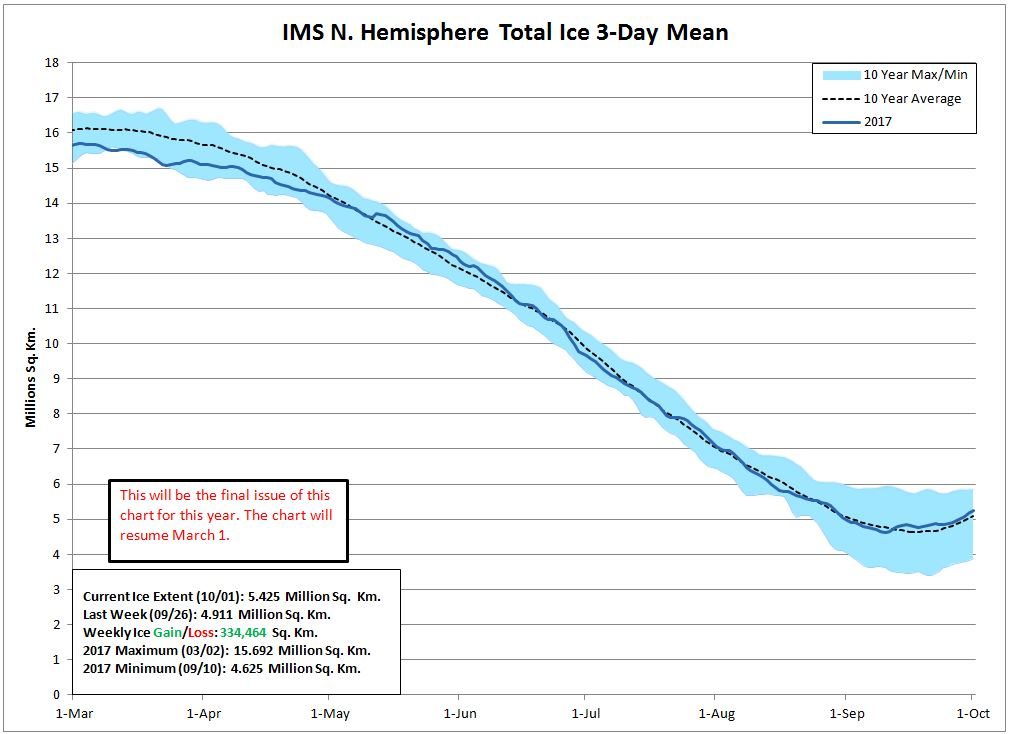
\includegraphics[width=\linewidth]{ims_data.jpg}
    \caption{ \label{fig:nat_ice} Sea and Lake Ice coverage of IMS data using 4 KM resolution. Ice coverages are calculated using a three day running mean from March until September each year. Blue border displays maximum and minimum values for the season. Areas are calculated using the Lambert Azimuthal Equal Area Projection with a WGS84 Datum. \cite{nat_ice}}
  \end{minipage}
\end{figure}
%

\subsection{Past work}

Flashforward to the appearance of the main Iphone in June 2007, the start of the cell phone insurgency. One year after, in July 2008, the Apple App Store was propelled. It included 552 applications and 135 of them were free. After two months, the App Store's most prominent rival was discharged, the Android Market. These days, a great many people know the Android Market as Google Play. After the arrivals of these two mammoths, the Windows application store propelled in October 2010 and was trailed by the Amazon application store in March 2011. The development and advancement of portable applications have not backed off. Information assembled from Nielsen demonstrated that application clients 18 and more established invested 65 percent more energy in applications than they completed two years prior. In May of that equivalent year, Gmail turns into the primary independent application to hit 1 billion downloads.

Talking more about mobile technologies, Applications began as a stripped down, single-work program to keep running on the telephone and some have kept on being only that. Be that as it may, with advances in equipment and programming the pattern has moved back to having applications accomplish more. This has enabled individuals to supplant a few bits of tech with a solitary cell phone or tablet and, simultaneously, made the information from that gadget a lot more entire. What's more, that information, as opposed to the applications themselves, is the place the genuine world-changing force lies.

Portable application configuration is a solid help for understudy focused registering. By including visual and spatial information in a portable application, understudies can build up a 3-D execution which can furnish the versatile application clients with a virtual ordeal. The improvement of a versatile application for a chronicled cemetery gives a case of how to coordinate database data with visual and spatial information to accomplish s virtual experience. The contextual analysis introduced here, utilizing both Android and \gls{iOS} gadgets, incorporates three sections. At first, a current database was changed over for versatile application get to. This was trailed by plan coordination in help of the coveted versatile application highlights. At last, the incorporation of a picture display, with visual and spatial components, coordinated with the portable application, brought about a convincing versatile application, giving a virtual copy of a genuine visit to the recorded site.

Significant issues that portable innovation faces in its initial occasions are portrayed as underneath:

\begin{itemize}
  \item Geo-representation for little displays of cell phones was confined by a few specialized limitations, for example, - the little presentation size and goals, absence of preparing force and memory, and most basic the battery life. Besides, the versatile system transmission capacity was extensively lesser than that in settled systems.
  
  \item The ease of use of versatile Geo-perception arrangements was upset by insufficient Geo-representation. The causes were either the utilization of checked paper maps intended for a medium with various attributes or the creation of obscured and jumbled maps that fit an extensive screen, however not the little cell phone screen with lower goals.
  
  \item The low web speed with surprising expense of smart phones were one of the real issues that were looked by individuals creating applications.
\end{itemize}


%
\begin{figure}[ht]
  \centering
  \begin{minipage}{4.5in}
    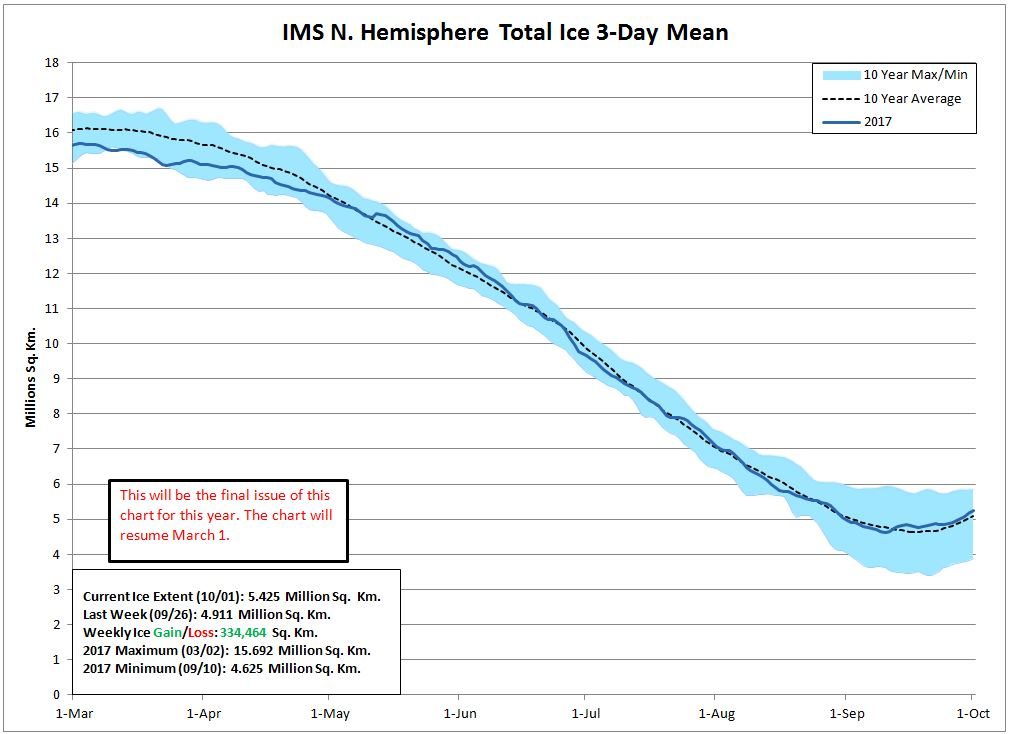
\includegraphics[width=\linewidth]{ims_data.jpg}
    \caption{ \label{fig:nat_ice} Sea and Lake Ice coverage of IMS data using 4 KM resolution. Ice coverages are calculated using a three day running mean from March until September each year. Blue border displays maximum and minimum values for the season. Areas are calculated using the Lambert Azimuthal Equal Area Projection with a WGS84 Datum. \cite{nat_ice}}
  \end{minipage}
\end{figure}
%

\subsection{Current scenario}

Notwithstanding late advances in pen-as well as contact empowered portable gadgets and the quick appropriation of these gadgets in ordinary life, we are a long way from utilizing the maximum capacity of cell phones in fulfilling the developing interest for visual access to information. Despite the fact that the plan space for versatile  information perception is developing out of ordinary practice [14], concentrated research endeavors have not yet risen.

Furthermore, Ongoing advancements in technology have demonstrated that systems of making and utilizing maps have changed fundamentally. The fields of getting, overseeing, investigating, intuitiveness and envisioning a lot of Geo-spatial information have seen exceptionally energetic and critical improvement throughout the most recent two decades and its quickly evolving. The ubiquity of hand held gadgets and portable Internet gives another stage to Geo-information. The cartographic presentation and plan for these little gadgets is a test because of their impediments.

Prior to the development of cell phones, information representation's house was the \gls{pc}, for the most part conveyed through programs and thick-customer applications. Be that as it may, when seen on savvy gadgets, information perceptions in PC-particular applications are hard to peruse, explore and utilize.

Yet, now, since portable applications are on a job, with having every one of the advancements that anybody needs to construct them, A bit of the present flexible applications in the market for data discernment are:

\begin{itemize}
  \item \gls{gis} Cloud Mobile Data Collection is a tool for today’s mobile devices which enables you to collect data and conduct field surveys faster and easier than ever before. Combined with powerful new custom mobile and web forms, the new Mobile Data Collection app can also be highly tailored for your mobile workforce and a wide variety of applications in minutes without any programming.
  
  %figure of the app screens hots - search mobile data collection app on app store and get screen shots
  
  \begin{figure}[ht]
  \centering
  \begin{minipage}{4.5in}
    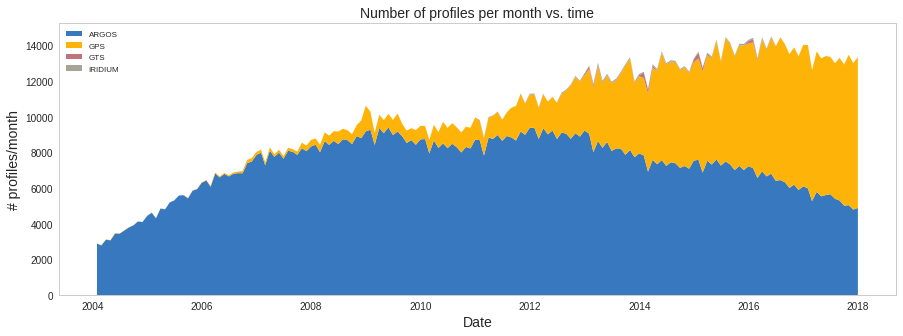
\includegraphics[width=\linewidth]{commTS.png}
    \caption{ \label{fig:commTS} Satalite Communication Type by month. Iridium floats also use the GPS system.}
  \end{minipage}
\end{figure}
  
  \item The "Spatial Agent" Mobile App has been created to exploit new capacities to picture this developing scope of spatial and transient advancement related information on versatile stages. The App shows a basic yet greatly ground-breaking way to deal with imagine a scope of open area spatial data sets through intuitive maps and graphs to take into account information representation at various scales and ranges. The methodology actually puts the globe in the clients hands and enables one to get to an expanding gathering of open space multisectoral data sets (counting at worldwide, provincial, and national levels) being produced for use by different improvement related foundations and governments over the world. So whether you are keen on water assets or environmental change, catastrophe administration or general advancement, this is an unquestionable requirement have App for you! The straightforwardness of utilization and abundance of data is certain to interest you – regardless of whether you are an understudy, advancement proficient, or a Minister!
  
  %figure of the app screens hots - search Spatial Agent app on app store and get screen shots
  
  \item \gls{gps} Tracks for Bike, Hike, Ski and Outdoor is ideal for outrageous competitors displays a totally new perspective of the world on your iPhone screen. It gives you that exact and vital data utilizing its 3D height show modified. Aside from the 3D show, it gives you a precise altimeter that shows your rise. Notwithstanding, you may discover a few challenges when attempting to match up it with Facebook or Twitter.
\end{itemize}

%figure of the app screens hots - search Maps 3D - Outdoor GPS app on app store and get screen shots
  
  \begin{figure}[ht]
  \centering
  \begin{minipage}{4.5in}
    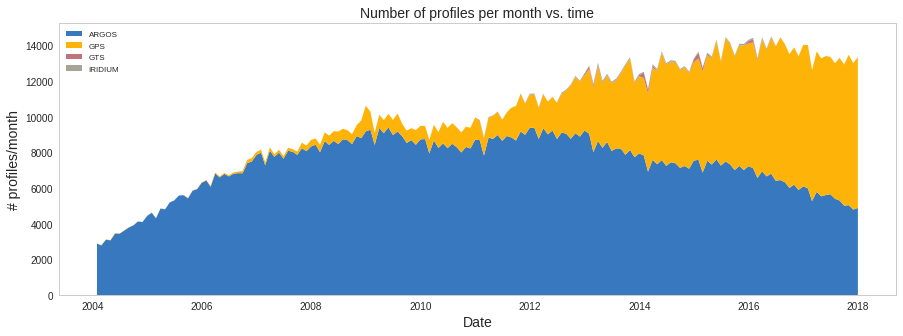
\includegraphics[width=\linewidth]{commTS.png}
    \caption{ \label{fig:commTS} Satalite Communication Type by month. Iridium floats also use the GPS system.}
  \end{minipage}
\end{figure}

\subsection{Future work for quick visualization and analysis of big data}

There were 4.77 billion versatile application clients in 2017, and it is anticipated there will be 5.07 billion portable application clients in 2019 (eMarketer). Of these billions of clients, 66 percent of clients apportion the vast majority of their opportunity between gaming, stimulation, news, and sports applications (Think with Google). In a report by App Annie, a normal US client spends more than 2.25 hours on applications and dispatches somewhere around 9 applications by and large. Included all together, US clients spend a little more than multi month in applications. As indicated by comScore's 2017 US Mobile App report, the 10 applications that command the US space are: Facebook, Youtube, Facebook Messenger, Google Search, Google Maps, Instagram, Snapchat, Google Play, Gmail, and Pandora.

%http://www.thinkebiz.net/mobile-apps-past-present-future/ 
% figures is at this url
% some graphs showing app market captured

\begin{figure}[ht]
  \centering
  \begin{minipage}{4.5in}
    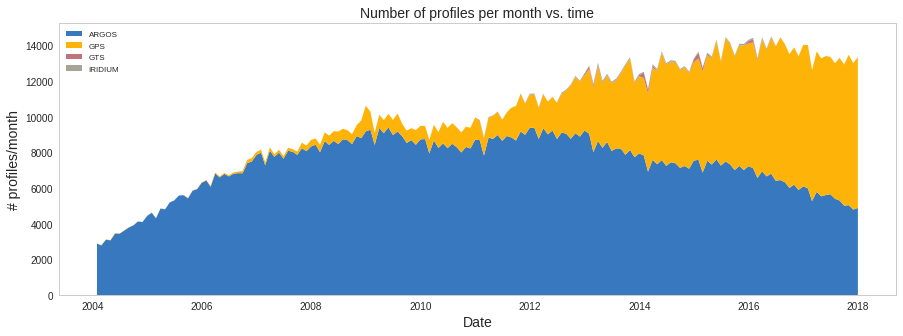
\includegraphics[width=\linewidth]{commTS.png}
    \caption{ \label{fig:commTS} Satalite Communication Type by month. Iridium floats also use the GPS system.}
  \end{minipage}
\end{figure}

Of everything portable applications, a standout amongst the most valuable perspectives might be the power it needs to develop your business. Applications enable you to traverse your day by day exercises, similar to messages, exercises, and mingling. So why not let it enable you to extend your business? One of the prominent misinterpretations is that applications are intended for huge brand organizations. In spite of the fact that, that isn't the situation. The greatest favorable position of having a versatile application is the immediate association with the clients. It includes the estimation of direct correspondence and comfort. It enables you to showcase new highlights, items, arrangements, or reliability programs truly into the palm of your gathering of people's hands. 

The energy of versatile application utilize resembles a projectile prepare that isn't backing off at any point in the near future. Ideally, you will bounce on the prepare – goal: development. \\ \\
\textbf{The Technology Trends}

The NGAC has pinpointed five innovation inclines that are encouraging, organizing, and driving improvement in geospatial advancements. They are: 

\begin{itemize}
  \item \textbf{The Real-Time Revolution} \\
  Albeit constant spatiotemporal information is currently being produced universally and its applications in research and business are across the board and quickly quickening, the capacity to ceaselessly make and cooperate continuously with this information is an ongoing marvel. This development is working as a center change specialist in geology, cartography, GIScience, and many related geospatial fields. It is significantly realigning conventional connections and structures; growing examination skylines; and changing the manners by which geographic information is presently gathered, mapped, demonstrated, and utilized in geology and science and society all the more comprehensively. This prompt collaboration among space and time remains today the hidden procedure that is creating the ebb and flow blast of combined spatiotemporal information, new geographic research activities, and heap versatile geospatial applications in governments, organizations, and society. 
  
  \item  \textbf{Scaling down of Technologies} \\
 The ability to make little and frequently cheap gadgets and sensors with remote availability is driving a blast of the Internet of Things (IoT). Scaled down and bring down cost sensors prompt an expansion in what, when, where, and how much information is gathered and, all the more vitally, the capacity to adjust the sensor to the particular information accumulation required. 
  
  \item  \textbf{Multiplication of New Mobile Geo spatial Sensor Platforms} \\
  The quick scaling down of innovations has made it practical to investigate new modalities for sensor dissemination, for example, little satellites (smallsats) and unmanned flying machine frameworks (UAS, or automatons) that can be quickly composed and sent with circles or flight ways custom fitted to the mission. These portable geospatial sensor stages extraordinarily extend the capacities of people, organizations, and governments to gather volumes of remotely detected information for various and mission-basic purposes, including catastrophe reaction, ecological checking, and open security. 
  
  \item  \textbf{Extending Wireless and Web Networks} \\
 Quicker and more extensive remote and web systems are starting to address, to a limited extent, the developing interest for enhanced techniques for information transmission and geospatial information conveyance to end clients. This is laying the basis for governments and shoppers around the globe to all the more comprehensively offer and utilize spatiotemporal information, including for constant applications. 
  
  \item  \textbf{Advances in Computing Capacity for Geospatial Research, Apps} \\
 Superior registering systems (counting CyberGIS) and distributed computing administrations (counting cloud GIS) are giving governments and others conductors through which they can all the more effortlessly and rapidly access and add to developing vaults of geospatial information, instruments, and administrations.
  
\end{itemize}

\section{Motivation of the VACYD research: crop yield data visualization}

\section{A short summary of the app development method and results}

Every day a great many versatile applications are distributed to the Google Play and Apple App Stores. A portion of these versatile applications are diversions, others are interpersonal organizations, and many are web based business applications. These applications, if professionally fabricated, ought to pursue a comparative portable application advancement process. At BHW, we have worked more than 350 web and portable applications and in this article I will diagram the technique, outline, and advancement forms we pursue. 

Each application is extraordinary and our philosophies are continually advancing, however this is a genuinely standard process when creating versatile applications. This versatile application advancement process regularly incorporates thought, methodology, plan, improvement, arrangement, and post-dispatch stages.

There are various methodologies, advancements, and programing dialects that can be utilized to fabricate a versatile application. Each with its very own qualities and inadequacies. Some may be less expensive to utilize, yet are less performant, though others may take more time to execute and be pointless excess. The most noticeably bad plausibility is expanding on a withering or untrustworthy innovation stack. In the event that you commit this error, you may need to remake your application or pay a premium for designers pushing ahead. That is the reason having a confided being developed accomplice that is prepared in settling on these choices is indispensable in this procedure.

For front-end improvement, there are essentially 3 approaches. They are stage particular local, cross-stage local, and crossover. Here is a concise outline of each methodology and a few articles that dig into each with more noteworthy subtle elements.

%figure of one example of each
%https://thebhwgroup.com/blog/mobile-app-development-process

\begin{itemize}
  \item \textbf{Platform-specific Native} \\ 
  Apps worked with this methodology are composed independently for every versatile stage. Code can't be reused among Android and iOS, yet these applications can be completely advanced for every stage. The UI can look altogether local (so it will fit in with the OS) and the application should work smoothly. This is frequently the most costly methodology, yet is extremely attempted and tried.
  
  \item \textbf{Cross-platform Native} \\ 
  Apps worked with this methodology have a few (or altogether shared) code, yet run locally. Regular advancements utilized for this are React Native, Xamarin, and Native Script. This is a decent center ground between the different methodologies in that it is more financially savvy, however can even now be upgraded and styled for every stage.
  
  \item \textbf{Hybrid} \\
 Cross breed applications are manufactured utilizing web innovations (HTML, CSS, Javascript) and are introduced by means of a local wrapper. This should be possible utilizing advancements, for example, Cordova, Phone Gap, and Ionic. This choice can be the least expensive, yet additionally shows some genuine troubles.
\end{itemize}

\\We have picked native application for the venture just due to following reasons:-

\begin{itemize}
  \item \textbf{Native fetures} \\ 
  There are numerous local highlights i.e. Camera, Document Directory access, Hardware Device Buttons, \gls{gpu} usage and so forth which you could conceivably approach on the off chance that you get your application created utilizing Hybrid innovation, contingent upon the structure that you embrace to create. On the off chance that your application is particularly far reaching and subject to local telephone capacity, at that point local application improvement will work best.
  
  \item \textbf{User experience} \\ 
  In the event that you are building up an application that requires some imaginative client encounter, don't think much and go for local application advancement. Cross breed application can never coordinate the level of imaginative client encounter that you get in local applications. \\
  So you see, now how rapidly you can choose whether to go for Hybrid application or Native application !! By and by I will dependably recommend to pick local application advancement except if you have a financial plan or time requirement.
  
  \item \textbf{Speed and Performance} \\
 Considering the application has been advanced for iOS or Android stage, this will appear in the execution levels. With local application advancement, everything is viewed as including the memory and battery of the cell phone. In addition to the fact that it is less demanding to execute motions, the code works quicker, new capacities will incorporate snappier, and the following of topographical area likewise stays basic.
 
\end{itemize}

\section{Literature review}